

\section{Introdução}
	\begin{frame}{}
		\centering
		\Huge \color{blue} \textbf{Introdução}
	\end{frame}

	\subsection{Motivação}	
	
		\begin{frame}{Motivação \cite{Diego}}
			
			\begin{itemize}
				
				\item \textbf{Metaheurísticas:} estratégias gerais alto-nível que guiam a busca por boas soluções através de busca local.
				
				\bigskip
				
				\item Métodos para problemas intratáveis ou difíceis são comuns na natureza e nas áreas de conhecimento.
				
				\bigskip
				
				\item O proposito é criar uma aplicação flexível para a resolução de problemas para facilitar futuros trabalhos a serem realizados.
				
			\end{itemize}
			
		\end{frame}
		
		
		
\section{Problema}
	\begin{frame}{}
		\centering
		\Huge \color{blue} \textbf{Problema da Coloração de Grafos}
	\end{frame}
	
	\subsection{Introdução}

	\begin{frame}{Problema} %Diego
		\begin{itemize}
        	\item Problema:
            
            \begin{itemize}

                \item Dado um grafo $G = (V, E)$, colorir os vértices de $G$ usando a menor quantidade de cores tal que para cada arco $(i, j) \in E$, os nós $i$ e $j$ tenham cores diferentes.

                \bigskip

                \item Uma $k$-coloração particiona $V$ em $k$ diferentes classes de cores, onde cada membro da classe tem a mesma cor.

                \bigskip

                \item O número cromático $\chi(G)$ de $G$ é o menor inteiro $k$ para o qual $G$ é $k$-colorável.

            \end{itemize}
            
            
            \bigskip
            
            
            \item Aplicação  \cite{Ziviani}:
            \begin{itemize}

                \item Escalonamento de variáveis em registradores de um processador.

                \bigskip

                \item Alocação de horários.

                \bigskip

                \item Alocação de cargas incompatíveis.

            \end{itemize}
            
        \end{itemize}
		
	\end{frame}
	
	\begin{frame}{Problema} %Diego
			
		\begin{figure}[!htb]
			\centering
			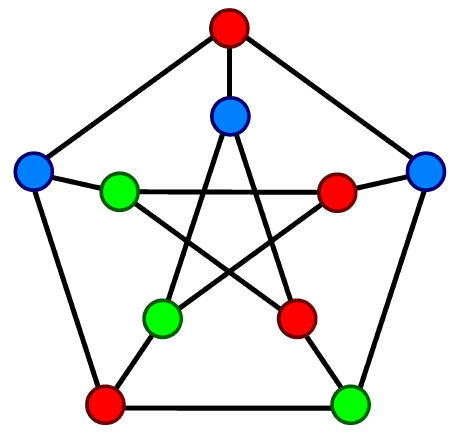
\includegraphics[width=0.6\textwidth]{corExemplo.png}
			\caption{$\chi(G)=3$}
			\label{fig:grafoProblema}
		\end{figure}
		
	\end{frame}


\section{Metodologia}
	\begin{frame}{}
		\centering
		\Huge \color{blue} \textbf{Metodologia de Desenvolvimento}
	\end{frame}

	\begin{frame}{Metodologia}
		
		\begin{itemize}
			
			\item Para solução do problema implementou-se os três métodos, Simulated Annealing, Hill Climbing e Algoritmo Genético.
			
			\bigskip
			
			\item Cada algoritmo possui seu arquivo de configuração.
			
			\bigskip
			
			\item Utilizou-se benchmarks populares desse problema para \\validação da execução.
            
			\bigskip
			
			\item Assim, analisou-se os resultados de cada instância com cada arquivo de configuração.
			
		\end{itemize}
			
	\end{frame}
		
		\subsection{Benchmarks}
		
			\begin{frame}[fragile]{Benchmarks}
				
				\begin{itemize}
					
					\item Foram utilizados para validação e análise dos métodos o conjunto de instâncias \textit{Graph Coloring Instances}\footnote{\url{http://mat.gsia.cmu.edu/COLOR/instances.html}} do Professor da Tepper School of Business da universidade Carnegie Mellon em Pittsburgh, Michael Trick's\footnote{\url{http://mat.gsia.cmu.edu/trick/index.html}}
					
					\bigskip
					
					\item Os arquivos se encontram em formato DIMACS.
					
					\bigskip
					
					\item O \textit{Center for Discrete Mathematics and Theoretical Computer Science} DIMACS\footnote{\url{http://dimacs.rutgers.edu/}} é um centro de pesquisa em matemática discreta, teoria da computação, algoritmos e métodos estatísticos criado em 1989 e sediado em Piscataway - Nova Jersey.
					
					
				\end{itemize}
				
			\end{frame}
			
			\begin{frame}[fragile]{Benchmarks -  Exemplo}
				
					
					{
						\footnotesize
						\begin{block}{}
							
							\begin{verbatim}
							c FILE: anna.col
							c Translated from Stanford GraphBase File: anna.gb
							o 11
							p edge 138 986
							e 1 36
							e 2 45
							e 3 74
							e 4 18
							e 5 36
							e 6 74
							e 6 45
							e 6 136
							e 6 36
							e 6 21
							e 6 18
							e 7 18
							e 7 116
							\end{verbatim}	
						\end{block}
					}
				
			\end{frame}
			
			
			\begin{frame}{Benchmarks}
				
				\footnotesize
				{	
					\begin{table}
						\centering
						\begin{tabular}{l|c|c|c|c|c}
							
							\textbf{Instância}       & \textbf{Vértices} & \textbf{Arestas} & \textbf{Densidade} & \textbf{Ótimo} & \textbf{Fonte}\\ \hline \hline
							mulsol.i.5.col  & 186      & 3973    & 0.231     & 31     &  REG  \\
							queen11\_11.col & 121      & 3960    & 0.545     & 11     &  SGB  \\
							queen13\_13.col & 169      & 6656    & 0.469     & 13     &  SGB  \\
						\end{tabular}
					\end{table}
				}	
                
				\bigskip
				
				\begin{itemize}
					
					\item Os arquivos são divididos por pelo seus criadores e cada um possui uma característica ou origem diferente.
					
					
				\end{itemize}
				
					\scriptsize
					{	
						\begin{table}
							\begin{tabular}{l|c}
								\textbf{Fonte} & \textbf{Descrição}                                                                                                           \\ \hline \hline
								SGB   & \specialcell{Grafos de Donald Knuth em Stanford GraphBase, são baseados em livros,\\ jogos de futebol, cidades dos EUA e Xadrez.} \\\hline
								REG   & Baseado em alocação de variáveis em registradores em códigos reais. \\
							\end{tabular}
						\end{table}
					}
					
			\end{frame}
		
        
        \subsection{Arquivos de Configuração}
        
			
			
			\begin{frame}[fragile]{Arquivo Configuração - Cabeçalho do Arquivo}
				
					
					{
						\footnotesize
						\begin{block}{}
							
							\begin{verbatim}
c Template de arquivo de configuração, 'c' equivale a um comentário

c Método de solução
m <ga|sa|hc>

c Parâmetros dos respectivos métodos 
							\end{verbatim}	
						\end{block}
					}
				
			\end{frame}
			
			\begin{frame}[fragile]{Arquivo Configuração - Simulated Annealing}
				
					
					{
						\footnotesize
						\begin{block}{}
							
							\begin{verbatim}
c Se for o Simulated Annealing

c Quanto menor, mais lento é o decaimento
beta <valor>
c Temperatura inicial
tinit <valor>
c Temperatura final
tfin <valor>
c Número máximo de iterações
samax <valor>
c Quantidade de vizinhos para explorar (Quantity of neighboors)
saqngb <valor>
							\end{verbatim}	
						\end{block}
					}
				
			\end{frame}
			
			\begin{frame}[fragile]{Arquivo Configuração - Hill Climbing}
				
					
					{
						\footnotesize
						\begin{block}{}
							
							\begin{verbatim}
c Se for o Hill Climbing

c Número máximo de iterações
hcmax <valor>
c Quantidade de vizinhos para explorar (Quantity of neighboors)
hcqngb <valor>
							\end{verbatim}	
						\end{block}
					}
				
			\end{frame}
			
			\begin{frame}[fragile]{Arquivo Configuração - Algoritmo Genético}
				
					
					{
						\footnotesize
						\begin{block}{}
							
							\begin{verbatim}
c Se for Genetic Algorithm

c Porcentagem de retorno do Melhor individuo.
taxaMelhorIndividuo <valor>
c Tamanho da populacao em cada iteracao
tamanhoPopulacao <valor>
c Quantidade de gerações de filhos em cada iteração da população
quantidadeGeracoes <valor>
c Porcentagem de aceitação da mutação, ou seja, se o valor
  cfor 0.8, 80% dos inivíduos serão mutados
mutacaoAleatoria <valor>
c Porcentagem para o uso dos métodos de seleção dos pais
  c caso for definido 0.8, 80% será feito com o método do torneio e
  c 20% será realizado com Elite
metodoSelecao <valor>
							\end{verbatim}	
						\end{block}
					}
				
			\end{frame}
        
        
        
        
        
		\subsection{Scripts Extras}
		
			\begin{frame}{Scripts Extras}
				
				\begin{itemize}
					\item Foram utilizados três \textit{scripts} básicos para auxiliar na execução dos métodos e análise estatísticas e visualização de seus resultados, são eles:
					
					%\bigskip
					
					\begin{itemize}
						\item \textit{\textbf{Script Shell:}} utilizado para coordenar de forma autonômica as várias execuções de cada instância do \textit{benchmark} para cada arquivo de configuração.
						
						\bigskip
						
						\item \textit{\textbf{Script R:}} utilizado para leitura seguida de tratamento do arquivo saída das execuções, gerando \textit{boxplots} para análise estatística dos resultados, possibilitando uma comparação entre as duas metaheurísticas.
						
						\bigskip
						
						\item \textit{\textbf{Script DOT:}} utilizado para gerar a representação gráfica do grafo colorido.
					\end{itemize}
					
				\end{itemize}
				
			\end{frame}
            
            
            